% libroResMat2
% Copyright (C) 2020  J.M. Perez Zerpa, et. al.
%
% This program is free software: you can redistribute it and/or modify
% it under the terms of the GNU General Public License as published by
% the Free Software Foundation version 3 of the License.
%
% This program is distributed in the hope that it will be useful,
% but WITHOUT ANY WARRANTY; without even the implied warranty of
% MERCHANTABILITY or FITNESS FOR A PARTICULAR PURPOSE. See the
% GNU General Public License for more details.
%
% You should have received a copy of the GNU General Public License
% along with this program.  If not, see <http://www.gnu.org/licenses/>.

\section{Estabilidad global estructuras}
A continuación se hace una breve mención a la estabilidad global de estructuras. Hasta esta sección se presentaron conceptos de estabilidad que comprenden el comportamiento de componentes individuales. Dichos conceptos se pueden llevar al estudio de la estabilidad de ensamblajes de componentes, es decir la estabilidad de sistemas estructurales completos.

\subsection{Sistemas resistentes de esfuerzos laterales}
En el contexto de estructuras de edificación, se puede definir el concepto de sistema resistente de esfuerzos laterales como aquella parte de la estructura que tiene como función resistir las cargas laterales que puedan ser aplicadas sobre la estructura y llevar dichas cargas al suelo.

Un paso clave en la definición de la estructura de una edificación es identificar el sistema resistente de esfuerzos laterales. El mismo se puede componer de pantallas, núcleos o pórticos entre otros. No todas las columnas verticales tienen porqué integrar el sistema resistente de esfuerzos laterales; este puede ser el caso en la medida que dichas columnas no tengan la rigidez necesaria para tomar esfuerzos laterales o que las conexiones que las vinculan al resto de la estructura no permitan que participen de dicho sistema resistente.

\begin{figure}[htb]
  \centering
  %\width{0.6\textwidth}
%  \includegraphics[width=0.95\textwidth]{figs/UT7/Esquema_de_nucleos.png}
	\caption{Sistemas Resistentes de Esfuerzos Laterales. Izquierda: esquema en planta de planos resistentes. Derecha: Alzados de distintas opciones de planos resistentes.}
	\label{fig:EsqNucleos}
\end{figure}

Se deben definir sistemas resistentes de esfuerzos laterales de manera de poder soportar esfuerzos laterales en cualquier orientación y también esfuerzos laterales con excentricidades arbitrarias. Esto lleva a requerir para una estructura al menos tres planos verticales resistentes no concurrentes como mínimo. No obstante, basadándose en el criterio de robustez estructural, es decir que un fallo localizado en la estructura no genere un daño desproporcionado en la misma, se debería evitar tener una situación en la cual un fallo local saque de servicio a uno de los planos resistentes y la estructura pasa a tener una sistema resistente lateral insuficiente.


\subsection{Amplificación de Efectos Globales}

Las normas actuales de diseño de estructuras de tipo edificación tanto de hormigón como de acero requieren que se evalúen los efectos de segundo orden esperados cuando la estructura se esté aproximando a su máxima capacidad resistente. Esto incluye tanto los efectos de segundo orden a nivel de componentes (i.e. P-$\delta$), así como los efectos de segundo orden globales (i.e. P-$\Delta$).

A continuación presentamos un resumen del tipo de enfoque que se presenta en la norma europea para la amplificación de efectos globales en estructuras de tipo edificación de hormigón (i.e. EN 1992-1-1). Más precisamente, se justificarán algunas de las expresiones presentadas en el Anexo H de dicha norma.

Considere una estructura compuesta de un pórtico traslacional 2-D el cual arriostra una serie de columnas bi-articuladas. Esta estructura busca simular edificio de una planta, donde el pórtico actúa como sistema resistente lateral.

\begin{figure}[htb]
  \centering
  \def\svgwidth{0.8\textwidth}
  \input{figs/UT7/globales.pdf_tex}
	\caption{Estructura de pórtico traslacional arriostrando columnas.}
	\label{fig:globales}
\end{figure}

La estructura tiene cargas verticales gravitatorias y una cierta carga lateral que puede provenir por ejemplo del efecto del viento.

Se propone realizar un análisis simplificado y aproximado del comportamiento de la estructura. En dicho análisis, se cambia el pórtico traslacional por un resorte lateral con igual rigidez lateral ($K_{p}$) que dicho pórtico.

\begin{figure}[htb]
  \centering
  \def\svgwidth{0.6\textwidth}
  \input{figs/UT7/globales2.pdf_tex}
	\caption{Resorte equivalente a pórtico traslacional arriostrando columnas.}
	\label{fig:globales2}
\end{figure}

El único grado de libertad de la estructura pasa a ser el desplazamiento lateral del piso superior ($u$). Se puede, por lo tanto, expresar la energía potencial total como función de dicho grado de libertad.

Se debe observar que cuando los extremos superiores de las columnas se mueven $u$ hacia el costado, dichos extremos descienden una cantidad $w(u)=H-\sqrt{H^2-u^2}$. Este descenso puede ser aproximado a orden dos, Maclaurin de por medio, como $w(u)=u^2/(2H)$.

La energía potencial total resulta por lo tanto:

$$\Pi(u)=K_p \frac{u^2}{2} -\sum_{i=1}^n P_i w(u) - F_H u$$

Substituyendo el descenso $w(u)$ por su expresión aproximada en función de $u$ y notando que es igual para todos los puntos de aplicación de las cargas $P_i$:

$$\Pi(u)=K_p \frac{u^2}{2} -\frac {u^2}{2H} \sum_{i=1}^n P_i - F_H u$$

Podemos evaluar por lo tanto el equilibrio de la estructura estudiando la condición de $\nabla \Pi(u)=0$ y la estabilidad del sistema estudiando la derivada segunda de $\Pi(u)$ en los puntos de equilibrio.

$$\frac{d \Pi(u))}{d u} = \left(K_p-\frac{\sum_{i=1}^n P_i}{H}\right)u - F_H = 0$$

Se debe reconocer que si se hubiera analizado la estructura linealmente, el desplazamiento lateral de equilibrio hubiera sido igual a $u^{(0)}=F/K_p$.

En adelante se denominará la carga vertical total sobre la estructura como $P_{tot}=\sum_{i=1}^n P_i$. A partir de la ecuación anterior se deduce que el desplazamiento lateral aproximado de segundo orden es igual a:

$$u=\frac{F_H}{K_p - P_{tot}/H}$$

Se procede a evaluar la estabilidad de los equilibrios por medio del estudio de la derivada segunda de la energía potencial total:

$$\frac{d^2 \Pi(u))}{d u^2} = K_p-\frac{P_{tot}}{H}$$

El equilibrio se tornará crítico (i.e. la estructura pasará de ser estable a inestable) cuando dicha derivada segunda se anule:

$$\left.\frac{d^2 \Pi(u))}{d u^2}\right|_{cr} = K_p-\frac{P_{tot,cr}}{H}=0$$

De donde se deduce que la carga vertical total crítica es igual a:

$$P_{tot,cr} = K_p H$$

Usando esta expresión de carga crítica, se puede expresar la deformación lateral aproximada de segundo orden de la siguiente manera:

$$u=\frac{u^{(0)}}{1 - P_{tot}/P_{tot,cr}}$$

Es decir, el sistema resistente lateral se desplazará lateralemente más cuanto mayor sean las cargas verticales totales relativas a la carga vertical crítica total de la estructura.

La norma EN 1992-1-1 presenta en el anexo H las siguientes expresiones equivalentes a las deducidas en esta sección:

\begin{figure}[htb]
	\centering
	%\width{0.6\textwidth}
	AGREGAR FIGURA
%	\includegraphics[width=0.7\textwidth]{EN_Pcrit.png}
	\caption{EN 1992-1-1, Anexo H. Carga crítica Global para sistemas resistentes laterales con deformación lateral de tipo distorisión.}
	\label{fig:EN_Pcrit}
\end{figure}

Para poder reconocer la carga crítica dada el anexo G, se debe reconocer que $\Sigma S$, la fuerza lateral soportada por el pórtico dividida por el ángulo de distorsión lateral ($\gamma = u / H$) del pórtico, es igual a:

$$ \Sigma S = \frac{F_H}{\gamma} = \frac{K_p u}{u/H} = K_p H  $$

A partir de lo cual, coinciden la carga crítica deducida y el valor propuesto por la norma. 

\begin{figure}[htb]
	\centering
	AGREGAR FIGURA
%	\includegraphics[width=1\textwidth]{EN_amplificacion_Global.png}
	\caption{EN 1992-1-1, Anexo H. Amplifiación de efectos laterales globales.}
\label{fig:EN_Pcrit}
\end{figure}

El Anexo H de la norma EN 1992-1-1 cubre casos más complejos que el presentado en esta sección, además de tomar en cuenta las particularidades del comportamiento material del hormigón armado, pero fundamentalmente aplica conceptos de estabilidad no más sofisticados que los vistos en esta sección.






\section{Puntos críticos e imperfecciones} \label{sec:puntoCritico}



\subsection{Tipos de Sistemas Estructurales} 

En esta sección se realiza una breve introducción al concepto de punto crítico a través del estudio de un conjunto de sistemas estructurales formados por barras rígidas unidas por articulaciones y/o resortes elásticos lineales (de desplazamiento y/o de giro). Para cada estructura y sistema de cargas se muestran las curvas de carga-desplazamiento para la estructura sin imperfecciones (curva que parte del origen en color negro) y con imperfecciones geométricas (curvas que presentan un desplazamiento para carga nula en color azul). Los tramos de trazo continuo representan equilibrios estables mientras que los tramos discontinuos puntos de algún tipo de inestabilidad. La presente sección está basada en \citep{Bazzano2017}.



El estudio de estabilidad elástica mediante el prinicipio de mínima energía potencial total puede realizarse tanto en estructuras discretas como continuas. La diferencia entre un tipo de estructuras y el otro es el espacio $\mcU$ donde se busca el mínimo.

En el caso de estructuras continuas, la configuración deformada de la estructura $\bfu$ se expresa mediante una o más funciones. Al trabajar con las ecuaciones en el continuo se puede decir que la estructura tiene infinitos grados de libertad o que $\mcU$ es un espacio de dimensión infinita, mientras que al trabajar con métodos como por ejemplo el MEF, la solución vive en un espacio $\mcU^h$ de funciones de dimensión finita, con la dimensión dada por el número de grados de libertad y las funciones de interpolación utilizadas \citep{Hughes1987a}.


El problema de minimización de la energía potencial total en el caso de $\bfu$ continua escapa de las herramientas usuales de Cálculo Vectorial y cae dentro del campo de Cálculo Variacional. En este curso no se presentará un tratamiento formal de esta última rama del cálculo, pero sí se deducirán algunos resultados puntuales usando ideas asociadas al mismo.

Por otro lado, en el caso de estructuras discretas, la configuración deformada de la estructura $\bfu$ puede ser expresada mediante un número $n\in\mathbb{N}$ de valores reales. En este caso se dice que la estructura tiene $n$ grados de libertad o que $\mcU$ es un espacio de valores reales de dimensión finita como $\bbR^n$.

En los capítulos introductorios de \citep{Bazzano2017} se presentan y analizan varios ejemplos de sistemas estructurales discretos, que introducen de forma didáctica los distintos tipos de estabilidad que se puede observar en estructuras de todo tipo de porte. En la Sección~




\subsubsection{Bifurcación Simétrica Estable}

Una bifurcación simétrica estable corresponde a una situación en la cual una estructura alcanza un punto crítico y a partir de ese punto, su curva de carga-desplazamiento se bifurca en varias ramas: una inestable y otras dos estables.

El pandeo de columnas elásticas pertenece a esta categoría. En la Figura\autoref{fig:discreto11} se puede ver una versión discreta de ese tipo de estructura. En estos casos, al alcanzarse la bifurcación las estructuras logran mantener la carga aunque sea con grandes deformaciones (ej. columna elástica en compresión). En la Figura\autoref{fig:critico1} se muestra la curva carga-desplazamiento correspondiente. Notar que estas estructuras no son sensibles a imperfecciones, siempre y cuando el comportamiento material permanezca elástico.
\begin{figure}[htb]
	\centering
	\subfloat[Esquema de estructura]{
		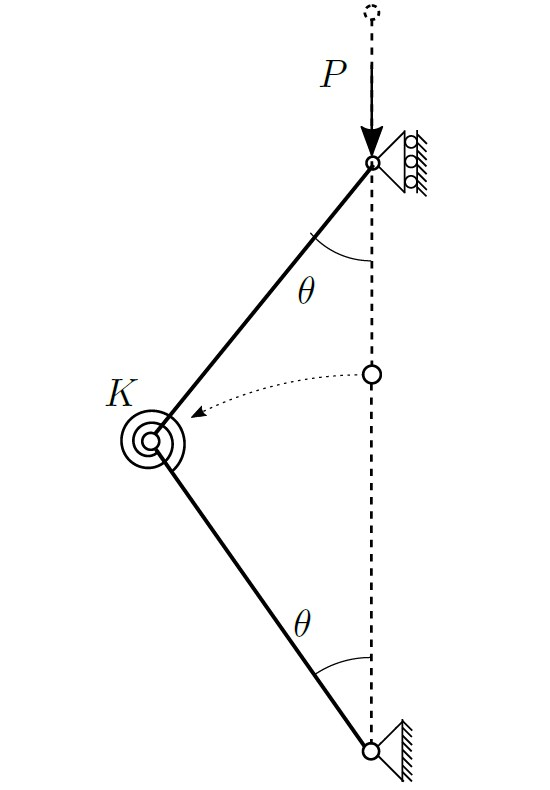
\includegraphics[width=0.25\textwidth]{Discreto1}
		\label{fig:discreto11}}
	\hspace{1em}
	\subfloat[Curva carga-desplazamiento]{
		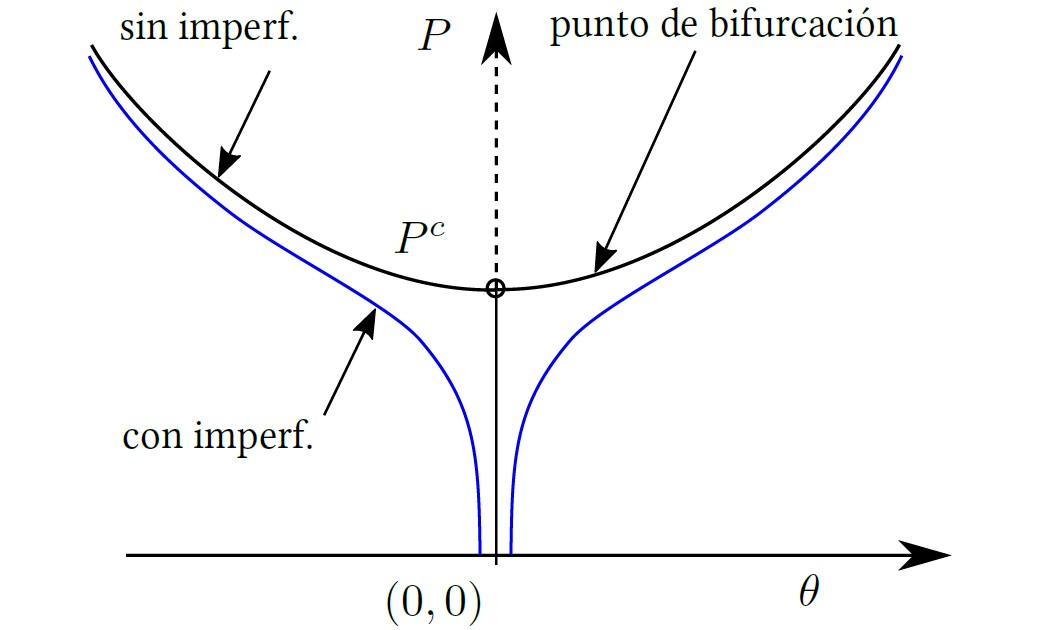
\includegraphics[width=0.55\textwidth]{Puntocritico1}
		\label{fig:critico1}}
	\caption{Estructura con comportamiento de bifurcación simétrica estable}
	\label{fig:simetrica1}
\end{figure}

\subsubsection{Bifurcación Simétrica Inestable}

Este tipo de comportamiento se corresponde al de estructuras y cargas tales que, al alcanzarse la carga crítica, la curva de carga-desplazamiento se divide en varias ramas, todas inestables. La rama inicial (fundamental) es la única estable.

Las cáscaras esbeltas sometidas a compresión muestran este tipo de inestabilidad, ya que al alcanzar el punto de bifurcación pierden la capacidad de soportar la carga (ej. lata de aluminio en compresión). En la Figura\autoref{fig:discreto21} se muestra una estructura discreta que exhibe este comportamiento, la configuración de la estructura sin carga aplicada es representada por líneas punteada $(\theta = 0)$ mientras que en líneas sólidas se muestra la configuración deformada.

En el gráfico de la Figura\autoref{fig:critico2} se observa que el comportamiento de estas estructuras es considerablemente sensible a imperfecciones. En general, la carga máxima soportada por la estructura decrece al considerar imperfecciones geométricas. El resultado observado en este ejemplo pone en evidencia la importancia de este tipo de análisis en estructuras como cáscaras.
\begin{figure}[htb]
	\centering
	\subfloat[Esquema de estructura]{
		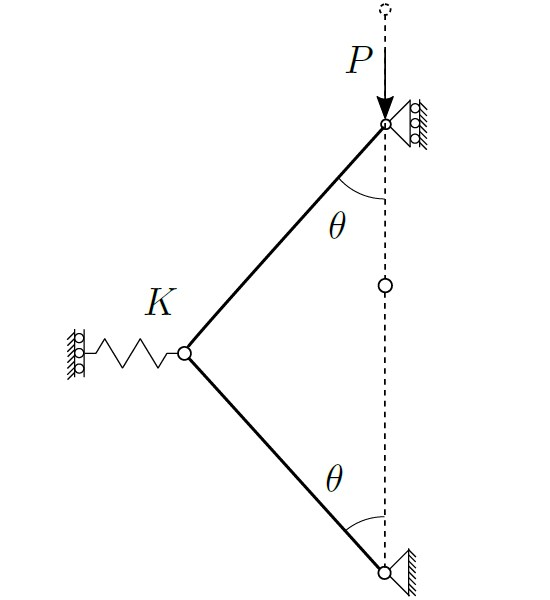
\includegraphics[width=0.3\textwidth]{Discreto2}
		\label{fig:discreto21}}
	\hspace{1em}
	\subfloat[Curva carga-desplazamiento]{
		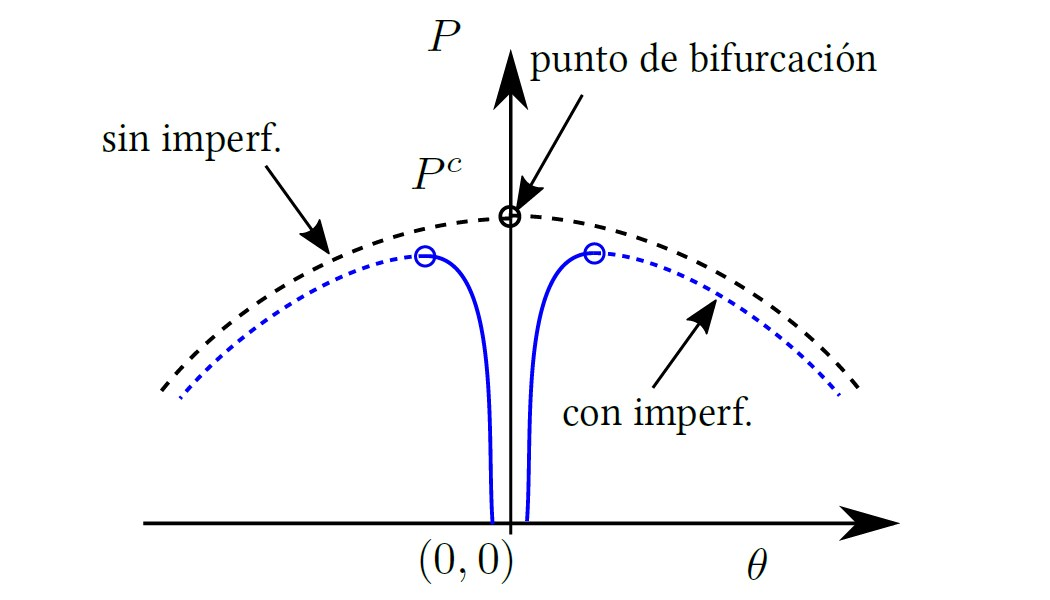
\includegraphics[width=0.55\textwidth]{Puntocritico2}
		\label{fig:critico2}}
	\caption{Estructura con comportamiento de bifurcación simétrica inestable}
	\label{fig:simetrica2}
\end{figure}

\subsubsection{Bifurcación Asimétrica}

Este tipo de comportamiento corresponde a situaciones en las cuales la estructura alcanza una configuración de equilibrio inestable en la cual la curva de carga-desplazamiento se divide en varias ramas: dos ramas inestables y una estable. En la
Figura\autoref{fig:discreto31} se muestra otro ejemplo de estructura con este comportamiento. En la Figura\autoref{fig:critico3} se muestran las curvas de carga-desplazamiento.

Considerando perturbaciones o imperfecciones hacia un lado la estructura se sigue una rama estable, mientras que con perturbaciones hacia el otro lado se sigue una rama inestable, con lo cual, se clasifica como inestable en general. Consecuentemente la estructura es considerada como sensible a imperfecciones.
\begin{figure}[htb]
	\centering
	\subfloat[Esquema de estructura]{
		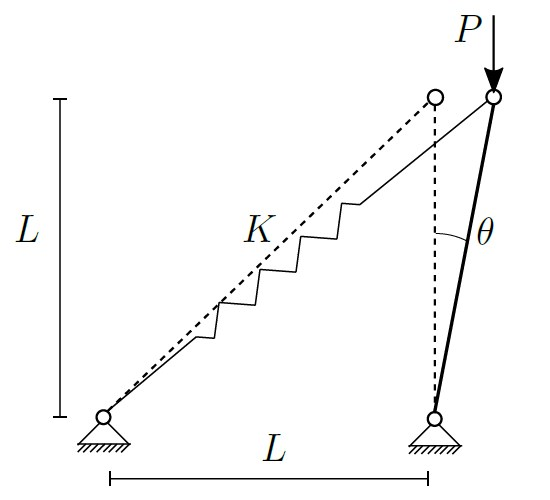
\includegraphics[width=0.3\textwidth]{Discreto3}
		\label{fig:discreto31}}
	\hspace{1em}
	\subfloat[Curva carga-desplazamiento]{
		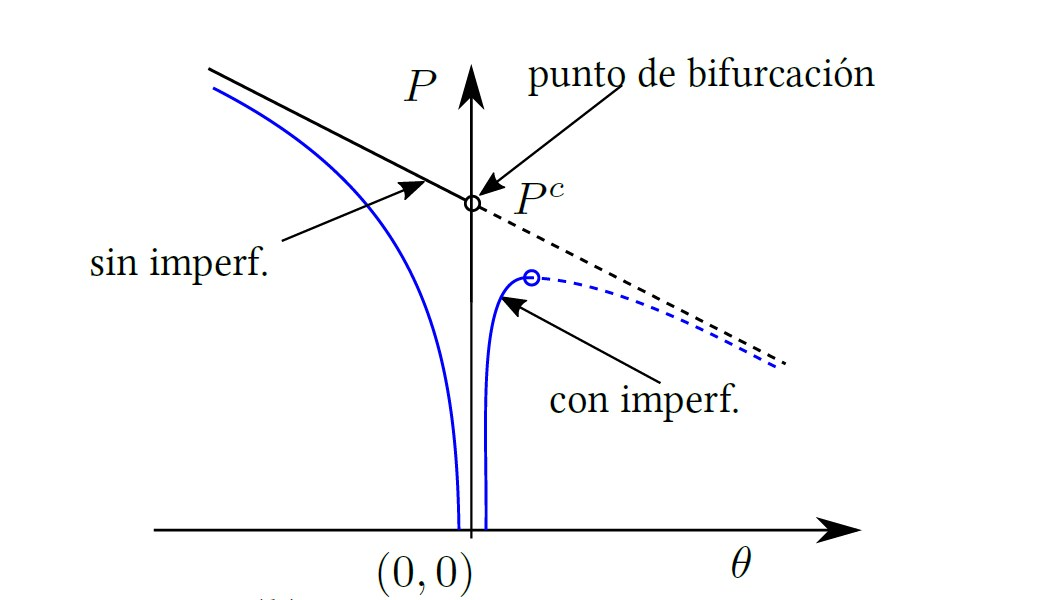
\includegraphics[width=0.55\textwidth]{Puntocritico3}
		\label{fig:critico3}}
	\caption{Estructura con comportamiento de bifurcación asimétrica}
	\label{fig:asimetrica}
\end{figure}




